\chapter{Falhas de Mercado}
\localtableofcontents 

Este capítulo é baseado nas notas de aula do curso, ministrado em 12/08/2023, e nos capítulos 12 (principal) e 13 de \textcite{cretì_fontini_2019}.

Por definição, uma firma tem poder de mercado se ela é capaz de discriminar preços total ou parcialmente. A forma como isso é feito pode mudar, mas essa característica permanece sempre. Por exemplo, um monopolista escolhe o preço e quantidade em que vende o produto diretamente, enquanto oligopolistas impactam o preço de equilíbrio estrategicamente via mudança nas quantidades ofertadas.

Nesta seção vamos discutir como competição imperfeita altera os resultados dos últimos capítulo e em que condições isso pode representar um problema para os procedimentos do mundo real.

\section{Competição Imperfeita}
Existem dois modelos principais modelos utilizados para estudar o tópico de competição imperfeita: Cournot e Bertrand. Ambos são chamados "jogos estratégicos", ou seja, as firmas se comportam como atores em um jogo no qual sempre preveem o comportamento da outra parte (assume-se racionalidade). Em todos esses modelos, tal qual apresentados aqui, são assumidos bens homogêneos.

\subsection{Modelo de Cournot}
Esse é o modelo prototípico de oligopólios. Aqui não será o foco derivar completamente o modelo e seus resultados (será coberto nas monitorias), apenas discutir as principais intuições.

Neste modelo cada firma opera como um monopolista na demanda residual das outras. Tome uma firma $i$, por exemplo. Ela escolherá uma quantidade para produzir, entendendo que sua escolha alterará o preço final do bem. Mais ainda, ela não se preocupa em atender a todo mercado, apenas a uma parcela de forma a maximizar seu lucro. 

Durante a escolha dessa quantidade ótima, ela leva em consideração que as demais firmas $-i$ também se deparam com um problema simétrico. Naturalmente, as firmas querem tomar a maior fatia do mercado para elas e, portanto, produzir mais. Entretanto, se todas produzirem muito o preço irá abaixar, não compensando o lucro que poderiam extrair da parcela ótima do mercado.

O resultado dessas forças atrativas e repulsoras de produção é chamado de equilíbrio de Cournot $(P^c,Q^c)$, que, via de regra, é tal que $Q^*>Q^c$ e $P^*<P^c$ onde $(P^*,Q^*)$ é o equilíbrio de mercado competitivo. 
\subsection{Modelo de Bertrand}
Esse é um modelo alternativo, mas igualmente importante e aplicável de monopólios, onde os incentivos são marginalmente diferentes. Ao invés de competirem na demanda residual (e, portanto, quantidades) como no modelo de Cournot, as firmas do oligopólio competem em preços.

Seja um preço fixo inicial $P_0$. Cada firma enfrenta o mesmo jogo (simétrico) e incentivos. A firma $i$ sabe que se abaixar o preço $P_0$ em uma quantidade infinitesimal $\varepsilon>0$ ela tomará todo o mercado para si (não há custos de transação) . Naturalmente, a firma $-i$ responderá abaixando o o preço $P_0$ em $2\varepsilon$, para roubar o mercado todo da firma $i$, e assim sucessivamente. 

O resultado dessa competição de preços é tal que o preço de equilíbrio $P^b$ será igual ao custo marginal da segunda firma mais eficiente i.e. $P^b=C_2'(Q^b)$. Em específico, no caso de um duopólio, esse resultado é idêntico ao de um equilíbrio competitivo.

\section{Leilões}
Leilões são uma das formas possíveis de se organizar um mercado que é interessante, em particular, por possibilitar recuperar preferências e demanda pelo bem comercializado. Esse é um campo enorme dentro de microeconomia e teoria econômica, mas que resumirei em alguns tipos abaixo:
\begin{itemize}
    \item \textbf{Leilões de Primeiro Preço:} Um leilão é realizado onde os apostadores não veem os lances dos seus adversários. O vencedor paga ao leiloeiro o valor de seu próprio lance.
    \item \textbf{Leilões de Segundo Preço:} Um leilão é realizado onde os apostadores veem os lances de seus adversários. Logo, o vencedor, por racionalidade, paga o valor muito próximo do segundo maior lance.
    \item \textbf{Leilões Uniformes:} Um leilão em que tanto oferta e demanda fazem preço. Pessoas escolhem vender um bem e outras escolhem comprá-lo. Desse processo surge um preço, tal qual em equilíbrio competitivo, mas todos entendem que sua decisão influenciará o preço final. Em Leilões Uniformes os "vencedores" irão receber/pagar o mesmo preço, independente do que tenham apostado.
    \item \textbf{Leilões Discriminatórios:} Similares à leilões uniformes, entretanto, cada apostador vencedor pagará o valor equivalente ao seu lance.
\end{itemize}
No contexto de eletricidade, é interessante pensar nessa estrutura de leilões, pois é assim que o processo de concessão de geração de energia costuma acontecer. Vamos, aqui, discutir em detalhe principalmente os últimos dois tipos de leilões e as implicações deles em cenários competitivos e - interessantes à esse capítulo - não-competitivos.

A Figura~\ref{fig:leil_comp} mostra os incentivos das empresas competitivas em ambas modalidades de leilão. Primeiro, note que a firma nunca tem incentivos à desviar do seu custo marginal para baixo pois, caso ganhe, ela estará pior do que caso tenha perdido (lucro negativo). Em leilões uniformes, as firmas também não tem incentivo à desviar para cima, pois as vencedoras vão receber o preço da firma marginal (na margem da vitória) independente disso, logo preferem aumentar a probabilidade de vencerem apostando seu custo marginal. Já em leilões discriminatórios, as firmas conseguem prever qual será o preço de equilíbrio e, portanto, as firmas que esperam vencer apostam nesse preço de equilíbrio para maximizar lucro. Portanto, sob mercados competitivos, ambos leilões levam aos mesmos resultados ainda que por mecanismos diferentes

\begin{figure}
    \centering
    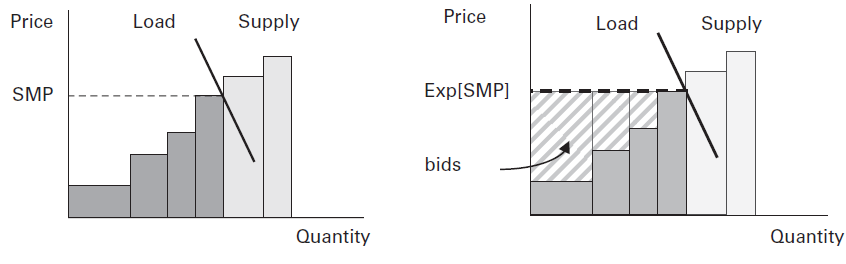
\includegraphics[scale=.5]{figure/leilao_comp.png}
    \caption{Diferenças de Leilões - Mercados Competitivos}
    \subcaption*{\footnotesize \textit{Nota:} A figura da esquerda mostra os incentivos das firmas em um sistema de leilão uniforme, já a figura da direita em um leilão discriminatório.}
    \label{fig:leil_comp}
\end{figure}

A Figura~\ref{fig:leil_ncomp_p}, por outro lado, mostra os incentivos para firmas não competitivas que estão exercendo poder de mercado (competindo) em preços. Note que o argumento anterior é exatamente válido aqui para todas as firmas exceto a marginal. Essa firma, em específico, tem incentivos a mentir e a reportar seu custo marginal apenas um $\varepsilon>0$ menor que a próxima firma na ordem de mérito para extrair lucro máximo. Em leilões discriminatórios, o mesmo argumento também vale para a firma marginal. Para as demais, entretanto, por ser mais difícil inferir o preço de equilíbrio, todas tem incentivo a apostar um pouco mais que seu custo marginal, mas não de forma generalizada à $P^*$ como no caso competitivo.

Caso as firmas compitam em volume, vemos na Figura~\ref{fig:leil_ncomp_p} que todas as firmas tem incentivo a mentir a sobre a quantidade em estoque/a ser entregue. Elas informam um valor menor e, assim, "empurram" a curva de oferta para esquerda, inflando os preços, por sua vez.

\begin{figure}[!b]
    \centering
    \begin{subfigure}{\textwidth}
        \centering
        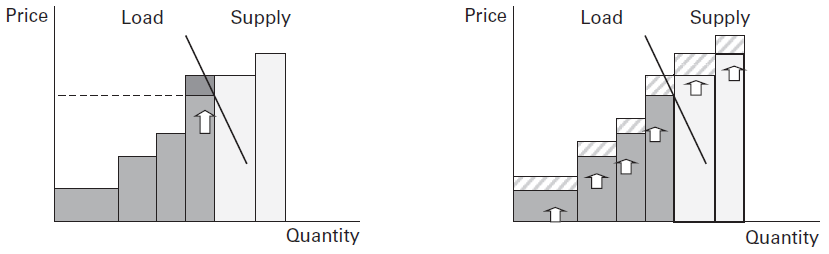
\includegraphics[scale=.5]{figure/leilao_ncomp_a.png}
        \smallskip
        
        \caption{Poder de Mercado em Preços}
        \label{fig:leil_ncomp_p}
    \end{subfigure}
    \smallskip
    
    \begin{subfigure}{\textwidth}
        \centering    
        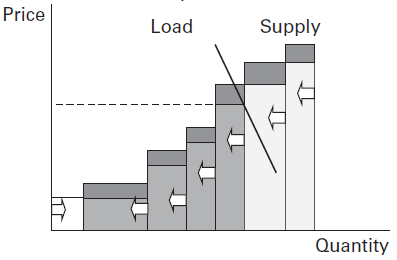
\includegraphics[scale=.5]{figure/leilao_ncomp_b.png}
        \caption{Poder de Mercado em Quantidades}
        \label{fig:leil_ncomp_q}
    \end{subfigure}
    \caption{Caption}
    \label{fig:leil_ncomp}
    \subcaption*{\footnotesize \textit{Nota:} No Painel (a), a figura da esquerda mostra os incentivos das firmas em um sistema de leilão uniforme, já a figura da direita em um leilão discriminatório. Já no Painel (b) a figura é referente a leilões uniformes, visto que discriminatórios com poder de mercado em volume é pouco sustentável do ponto de visto de incentivos.}
\end{figure}

\section{Medindo Competitividade}
Durantes as aulas foram apresentados dois índices comumente utilizados para medir o grau de competitividade de mercados: o \textit{Herfindahl-Hirschmann Index} (HHI); e o \textit{Pivotal Supplier Index} (PSI). Além das diferenças metodológicas, é importante notar que o HHI é utilizado em uma pluralidade de contextos, enquanto o PSI é específico da análise do setor de energia. No Capítulo 13 de \textcite{cretì_fontini_2019} também são discutidas outras possíveis formas de se mensurar concentração de mercados.

\subsection{\textit{Herfindahl-Hirschmann Index} (HHI)}
O HHI é definido como a soma dos quadrados dos \textit{market-shares} de $n$ empresas em um determinado setor i.e.:
\begin{align*}
    HHI=\sum_{i=1}^ns_i^2
\end{align*}
onde $s_i$ denota o \textit{market-share} da firma $i$.

É comum usar \textit{market-shares} expressas em termos percentuais para calcular o HHI ou, alternativamente, multiplicá-lo por 10.000. A Divisão Antitruste do Departamento de Justiça nos Estados Unidos (DOJ) usa os seguintes níveis:
\begin{itemize}
    \item $HHI<1000$ denota um mercado não-concentrado;
    \item $HHI\in(1000,1800]$ denota um mercado com baixa concentração;
    \item $HHI>1800$ denota um mercado concentrado (pouco competitivo)
\end{itemize}
No entanto, usar o HHI para avaliar a concentração em mercados de energia pode produzir resultados enganosos. Nesses mercados, como vimos, as fábricas normalmente têm restrições de capacidade. Isso implica diferentes estruturas de mercado podendo produzir diferentes
HHIs, mas afetando o preço de equilíbrio.

\subsection{\textit{Pivotal Supplier Index} (PSI)}
O PSI foi proposto por \textcite{borenstein1999market} e é uma
tentativa de incorporar o conceito de fornecedor marginal na mensuração do poder de mercado nos mercados de eletricidade. Este indicador examina se um determinado produtor ou usina é “pivotal” i.e. necessário para atender a demanda em um determinado momento, no sentido de que haverá um desligamento de carga sem a presença desta usina. O PSI pode ser definido como a razão de todas as horas (ou diferentes unidades de tempo) em que a usina foi pivotal por um determinado período. Por exemplo, se o período for um ano e a unidade de tempo for horas, o PSI da usina $i$ é:
\begin{align*}
    PSI_i = \frac{\sum_{j=1}^{8760}\mathbbm{1}\left[q^{dj}-\sum_{\substack{f=1\\f\neq i}}^nq_f^{max}\right]}{8760}
\end{align*}
onde $q^{dj}$ denota a carga na hora $j$ e $\mathbbm{1}[\cdot]$ é a função indicadora. Enquanto o HHI é uma medida da concentração geral do mercado, o PSI é uma medida de concentração do excedente de capacidade do sistema, ou seja, a possibilidade de igualar o total
oferta e demanda do sistema em qualquer período de tempo específico. 

Uma conclusão importante deste índice é que é possível que uma usina que não é despachada (esta à direita da curva) é importante para determinar poder de mercado, pois sua remoção do leilão pode implicar geração de usinas pivotais.